\subsection{Basic Algorithm}

In our protocol, a peer first tries to download the file from an origin web server.  If at some point one of the following conditions occurs, the download switches to a peer-to-peer swarming download:
\begin{enumerate}
\item First the client waits a maximum number of seconds $T$ after the start of a normal HTTP download, for the first byte of data to arrive.  This allows the system to decide quickly whether the origin server is over-burdened and switch to peer-to-peer if needed.   
\item Once the client gets some data from the server, then it monitors whether the download rate falls below a certain fixed threshold $R$ bytes per second over a window of time $W$.  If the origin server ever starts to serve slower (below $R$), the client switches to peer-to-peer delivery.
\end{enumerate}

Once a client decides to switch to peer-to-peer downloading, it may need to first lookup meta-data about the file to download.  To do so (if necessary), the client will calculate a hash value for the filename.  It will use this as a $key$ value in the DHT to retrieve the meta-data about the file.  After, peers randomly choose $b$ blocks of the file to download, and retrieve a list of peers who have those blocks.  The peer chooses one peer at random for each block, and downloads the block from that peer.  It then adds itself to the list of peers willing to share that block (see Fig. \ref{fig:download_all_steps}).  While it is attempting to contact peers for a block, in the meantime it attempts to download the block from the origin server, as well.  If peers download a file previously unknown to the system, then they update the data about the file (size, etc.) to its appropriate hash location in the DHT.  To combat the ``slow last block'' problem,  we download the last block from several peers, similar to how BitTorrent handles that problem\footnote{In reality, we download from $b$ peers at a time, including for the last $x$ blocks, i.e. if you have $b$ set to 10 and have 5 blocks left, each will be downloaded by 2 peers simultaneously, and so on down to the last block being downloaded by $b$ connections all redundantly}.

\begin{figure*}
  \begin{center}
    \subfigure[Peer downloads list of blocks]{\includegraphics[width=7cm]{description_pics/peer_step_1.png}}
    \subfigure[Peer downloads a list of peers which have a block]{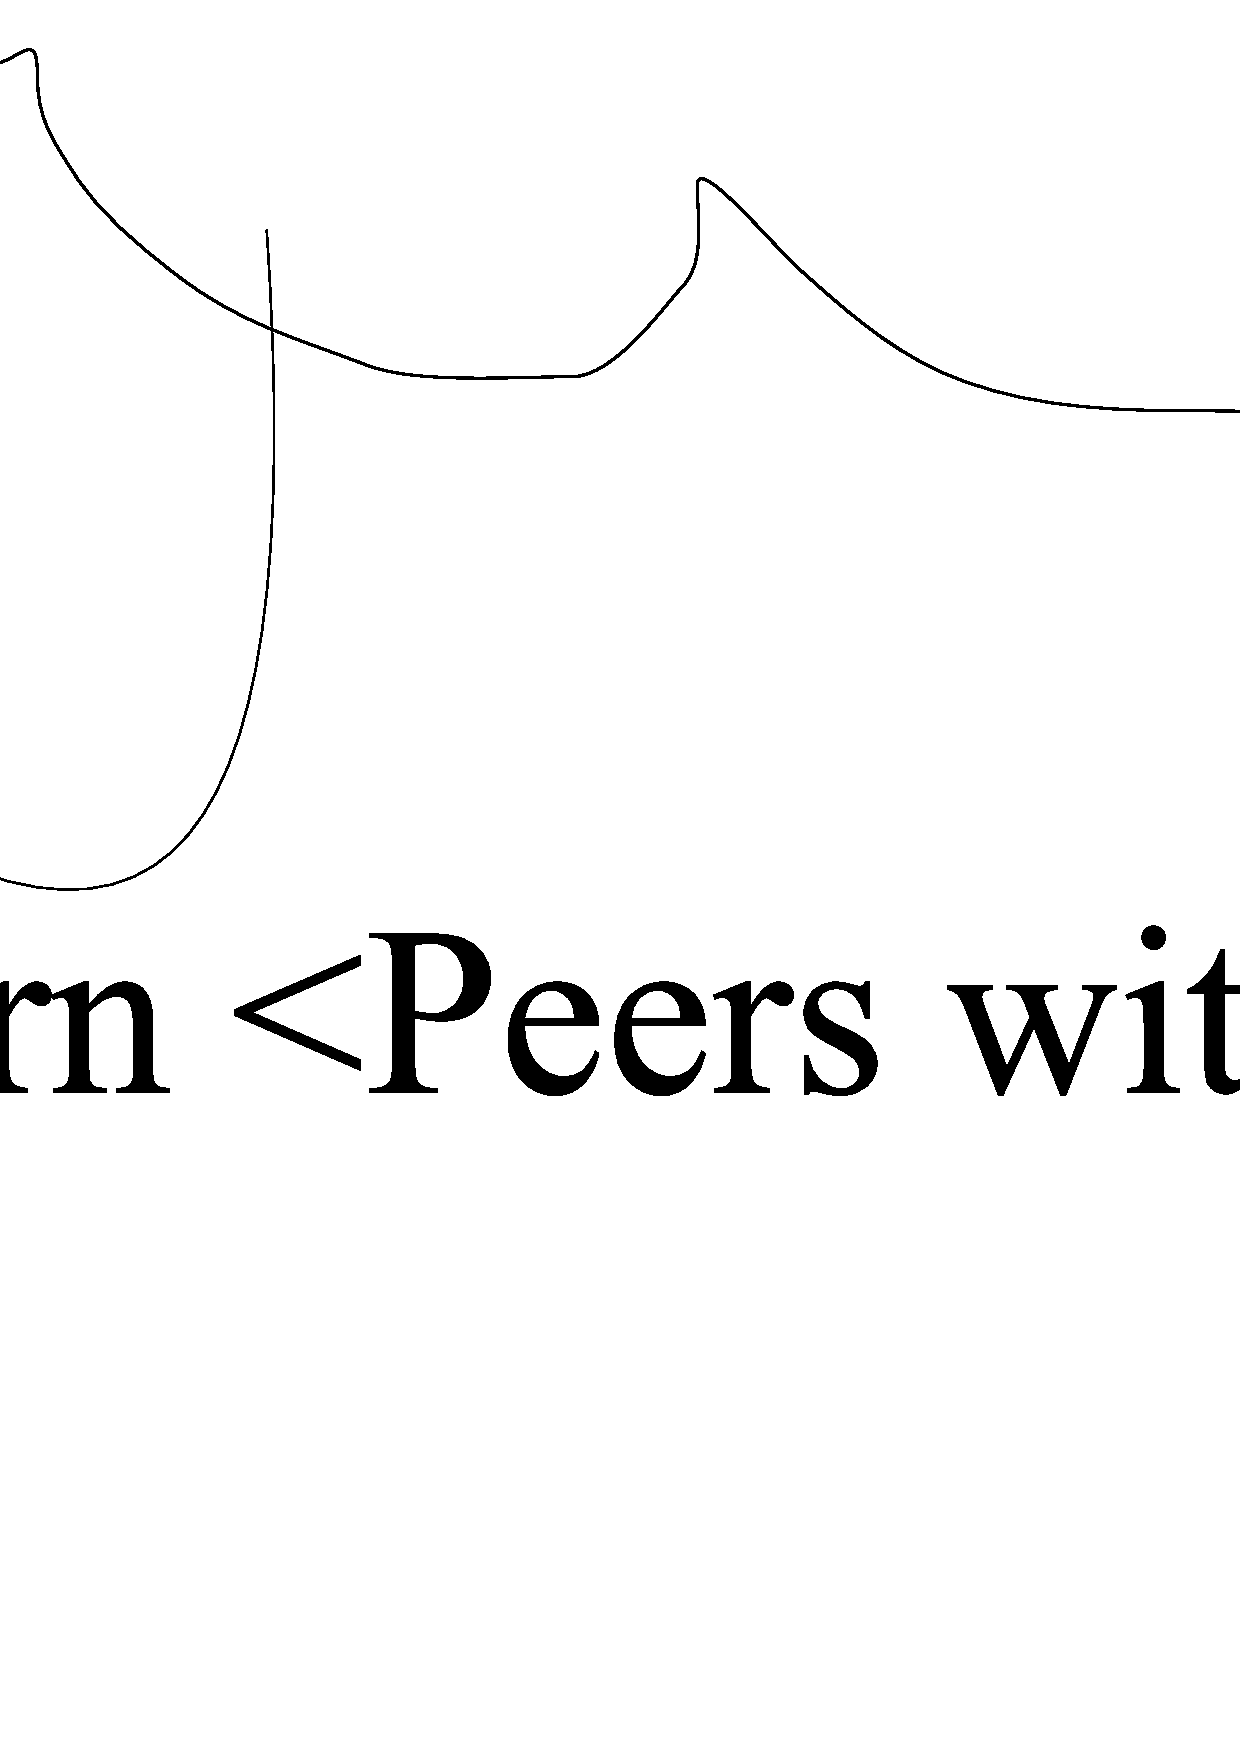
\includegraphics[width=7cm]{description_pics/peer_step_2.png}}
    \subfigure[Peer adds itself to list of peers who have that block]{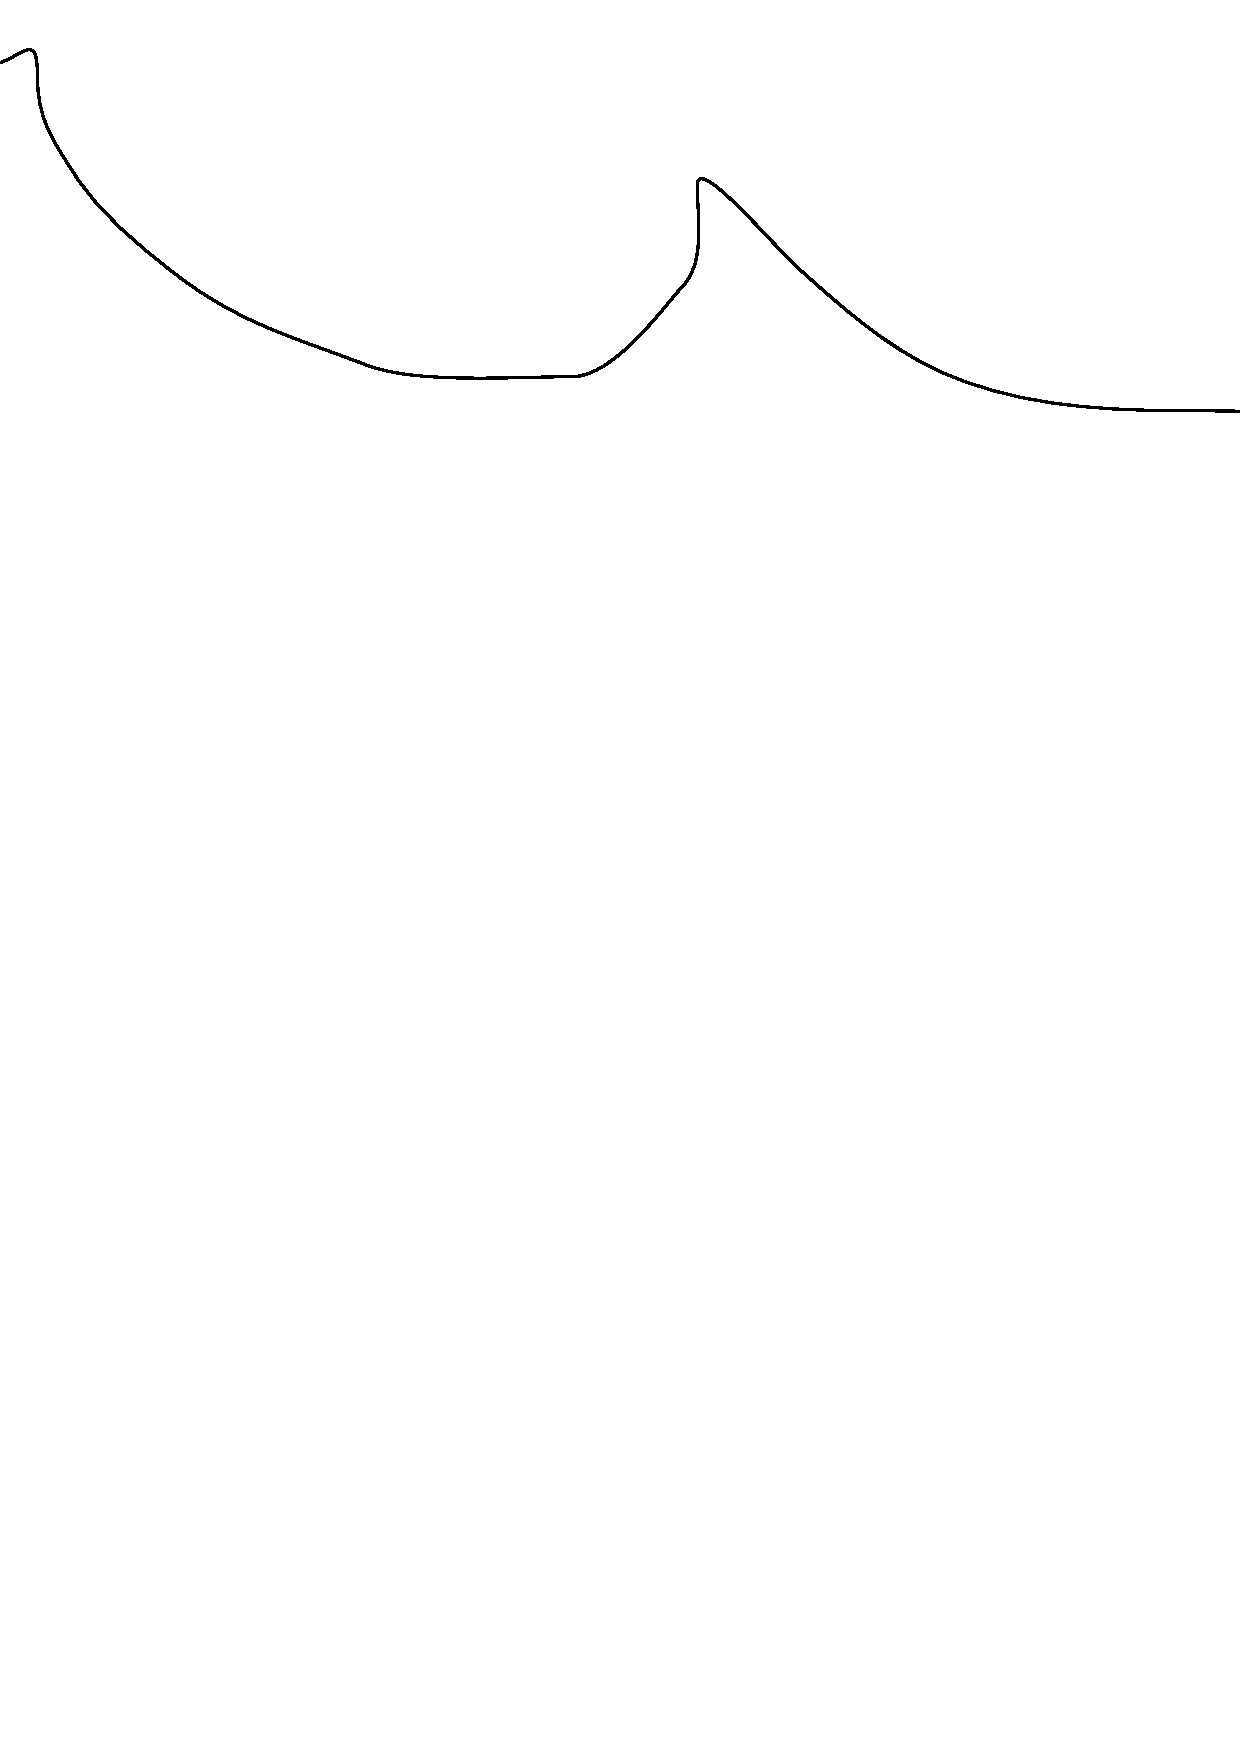
\includegraphics[width=7cm]{description_pics/peer_step_3.png}}
    \caption{Steps to accomplish a peer-to-peer-web download.}
    \label{fig:download_all_steps}
  \end{center}
\end{figure*}

